\documentclass{article}
\usepackage[top=20mm, right=20mm, left=20mm, bottom=25mm]{geometry}
\usepackage[utf8]{inputenc}
\usepackage{bbm}
\usepackage{mdwlist}
\usepackage{amsfonts}
\usepackage[T1]{fontenc}
\usepackage{mathptmx}
\usepackage[scaled=0.84]{beramono}
\usepackage[scaled=0.84]{helvet}
\usepackage{listings}
\usepackage{graphicx}

\title{Simple E-Voting System -- User Guide}
\author{Andreas Koch}

\lstset{
	basicstyle=\tt\small,
	showstringspaces=false,
	showtabs=false,
	tab= ,
	frame=shadowbox, 
	%numbers=left,
	%framexleftmargin=5mm, 
	frame=single,
	%numberstyle=\tiny,
	%numbersep=5pt
}


\begin{document}
\maketitle

\tableofcontents
\newpage

\section{Requirements}
The eVoting Software requires at least Java 1.7 to run, it was tested to work with Windows and Linux (Oracle JRE or JDK). All connection capabilities have been tested with IPv4 connect information.

\section{SimplevotingControlPanel}
The SimpleVotingControlPanel is a graphical interface for configuring and running all the different components of this software. To start it, navigate to bin\ directory and use this command (without linebreaks):
\begin{lstlisting}
java -cp .;..\lib\bcprov-jdk16-146.jar 
de.uni.trier.infsec.protocols.simplevoting.voterGUI.SimplevotingControlPanel
\end{lstlisting}
You should see the following window:\\
\begin{center}
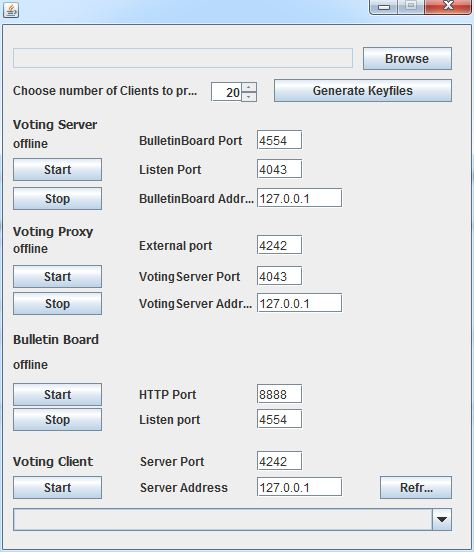
\includegraphics{./controlpanel.jpg}
\end{center}

\subsection{Selecting a directory}
First, you must select a directory where the keyfiles are located or to which you want to store generated keys to. Therefor press Browse and select a directory.

\subsection{Generating Keys and credentials}
In order to run eVoting server or clients you need to generate keyfiles first. If you already generated keyfiles, you can leave out this step, otherwise choose the number of keys to generate and press "Generate Keyfiles". Depending on the number of keys you chose, there will be following files created:
\begin{enumerate}
	\item Voters private keys (file suffix ".pri"), named voterXX.pri, whereat XX is a subsequent number starting from zero.
	\item Voters public keys (file suffix ".pub"), named voterXX.pub, whereat XX is a subsequent number starting from zero. Note: Corresponding public/private keys have same number.
	\item Servers key list (contains all voters public keys) named clients.evo
\end{enumerate}
Please note: The servers public and private key are currently included in the source code.

\subsection{Controlling VotingServer}
To run the eVoting server, select the port to listen for messages from voters or network proxy(\textbf{Listen Port}) as well as address and port to send casted ballots and the result to (\textbf{BulletinBoard Address / Port})
By pressing Start the server is started. Please make sure the bulletin board is running in order to access the election result.

\subsection{Voting Proxy}
As VotingServer only serially listens to one port, it might be necessary to enable multiple parallel client connections at one time. For doing this, there is Voting Proxy which can handle multiple connections to its external port and forwards messages to VotingServer. As configuration it takes the external port to listen to (\textbf{External Port}) as well as the voting servers connect information (\textbf{VotingServer Port / Address}). Voting Proxy does not have any graphical interface.

\subsection{Bulletin Board}
Bulletin Board is a simple HTTP Server, which accepts the ballots the Voting server casted, as well as the elections results, and makes them public available via HTTP. As configuration it takes the port whereat the webserver listens for GET requests (\textbf{HTTP Port}) and the port it listens for messages from eVoting Server (\textbf{Listen port})

\subsection{Voting Client}
If the selected directory contains public and private keyfiles, a voting client can be started from control panel. Therefor the file must be selected from the dropdown menu. As configuration it takes the connect information of the voting server (\textbf{Server Port / Address}). Please note: When using Voting Proxy, the clients are supposed to connect to the proxy!


\subsection{General information}
When using ControlPanel to start components of the software, each one is started within its own process and Java virtual machine to make sure, there is no interaction of the components beside the network channel. Of course the components are not required to run on the same physical machine.

\section{Starting Components without Control panel}
You can also start each component without the control panel using these commands:\\
\textbf{VotingServer}
\begin{lstlisting}
java -cp .;..\lib\bcprov-jdk16-146.jar 
de.uni.trier.infsec.protocols.simplevoting.VotingServerStandalone 
<path-to-clients.evo> <listen-port> <bulletin-board-address> <bulletin-board-port>
\end{lstlisting}
\textbf{VotingClient}
\begin{lstlisting}
java -cp .;..\lib\bcprov-jdk16-146.jar 
de.uni.trier.infsec.protocols.simplevoting.VoterStandalone
<path-to-publickey> <path-to-privatekey> <voting-proxy-address> <voting-proxy-port>
\end{lstlisting}
\textbf{HTTP BulletinBoard}
\begin{lstlisting}
java -cp .;..\lib\bcprov-jdk16-146.jar 
de.uni.trier.infsec.protocols.simplevoting.HTTPBulletinBoard 
<listen-port> <HTTP-server-port>
\end{lstlisting}
If no parameters are specified, the default ports 4554 for listen port and 8888 for webserver port are used.\\
\textbf{Network Proxy}
\begin{lstlisting}
java -cp .;..\lib\bcprov-jdk16-146.jar 
de.uni.trier.infsec.protocols.simplevoting.NetworkProxy
<listen-port> <voting-server-address> <voting-server-port>
\end{lstlisting}
If no parameters are specified, the default ports 4949 for listen port, 4242 for voting server port and 127.0.0.1 for voting server address are used.

\section{Voting server}
When running Voting Server, this graphical interface will open\\
\begin{center}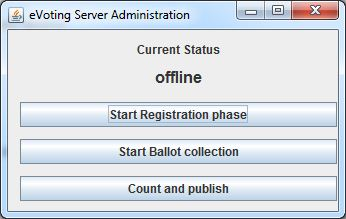
\includegraphics{./server.jpg}\end{center}
Initially the server is offline, which means it does neither accept clients registrations, nor ballot submissions. Note: The server actually does not store its state persistent. Once it is closed, all credentials and ballots get lost.
\subsection{Registration phase} By hitting the button \textbf{Start Registration phase} the server listens for registration messages. If a valid message is received, it decrypts it, generates credential for the voter and replies a message containing the credential encrypted with voters public key. In case of repetitions, the server will send the stored credential again.
\subsection{Ballot Collection} Once the server was switched to collection phase, it cannot switch back. In this phase, it listens for ballot submissions. Only registered clients, which have received a valid credential, can submit their vote. Every ballot that has been received will be sent to the bulletin board and made public available.
Note: Revoting policy is "last vote counts".
\subsection{Evaluation} Once \textbf{Count and public} is pressed, the server stops collecting votes. All ballots are now decrypted and counted. The result gets published to the bulletin board. It is not possible to switch back to ballot collection.

\section{Voting client}
When the Voting Client application is started, it looks like this:
\begin{center}
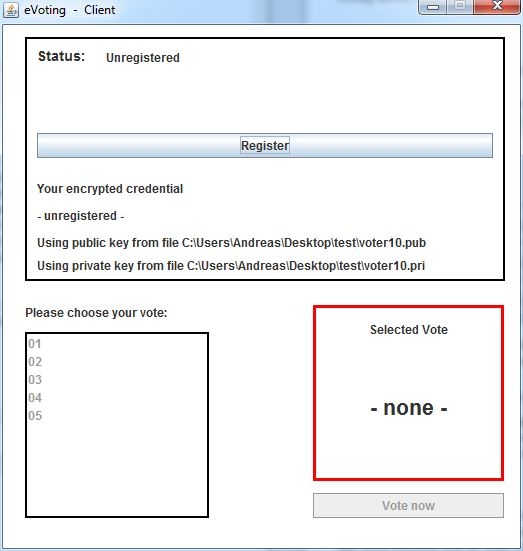
\includegraphics{./client.jpg}
\end{center}
As the voting protocol requires registration first, the client will be disabled except the \textbf{Register} button. Pressing it, the client will send a request for credentials to the server. If the server is running and is currently in registration phase, it will respond with the encrypted credential. 
Note: The client stores the credential locally. Once registered, the client can be closed and reopened later.
Once registered, the remaining controls get activated:
\begin{center}
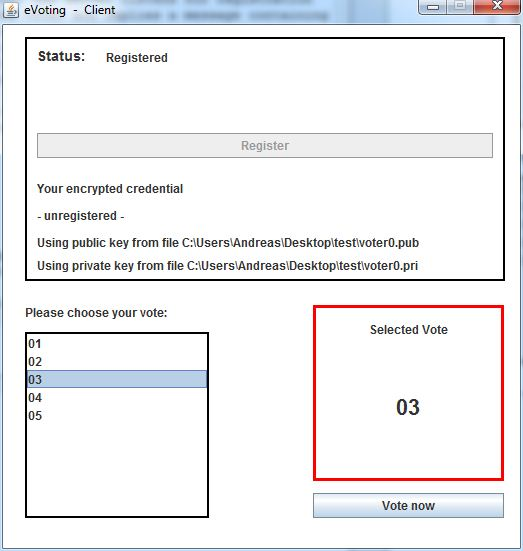
\includegraphics{./clientregistered.jpg}
\end{center}
By hitting \textbf{Vote now} the currently selected vote is encrypted with the credential and submitted to the server. Repeated clicks will cause one message per click, only the last vote is casted. You can vote as often as you want, as long as  the voting server is in ballot collection phase.

\section{Technical information}
This software uses BouncyCastle crypto provider to generate keys and perform cryptographic operations. For asymmetric crypto, it uses 1024 bits RSA. Currently, the client and server software expects the clients public and private key as files. 
These files should have following format:
\begin{itemize}
	\item Clients public key (.pub files) contain the binary representation of the RSA public key, encoded using ASN.1 encoding, defined in X.509 standard.
	\item Clients private key (.pri files) contain the binary representation of the RSA private key, encoded using ASN.1 encoding, defined in PKCS\#8 Standard
	\item Servers public Key list format
		\subitem First line: Public Key count
		\subitem One line per Key, containing the public key in ASN.1 (X.509) encoding represented as hexadecimal string.
\end{itemize}



% Format
% Was für wen

\end{document}
